\chapter{Conception et développement de l’application}
\label{chap:Chapter 3 title}
\section*{Introduction}

\hspace{16pt}Ce chapitre se concentre sur la conception et le développement de l'application. Nous commencerons par une description détaillée du flux de l'application, en expliquant comment elle guide les utilisateurs à travers ses différentes fonctionnalités. Ensuite, nous aborderons les choix technologiques majeurs, notamment l'utilisation de React pour l'interface utilisateur et Symfony pour le backend. Enfin, nous présenterons les diagrammes de conception utilisés pour visualiser et planifier l'architecture de l'application.

\newpage


\section{Description du flux de Chatbot}

\hspace{16pt}Le flux de l'application du chatbot pour la maison médicale se déroule en plusieurs étapes clés, organisées pour optimiser l'expérience utilisateur:

\begin{figure}[H] 
    \centering
    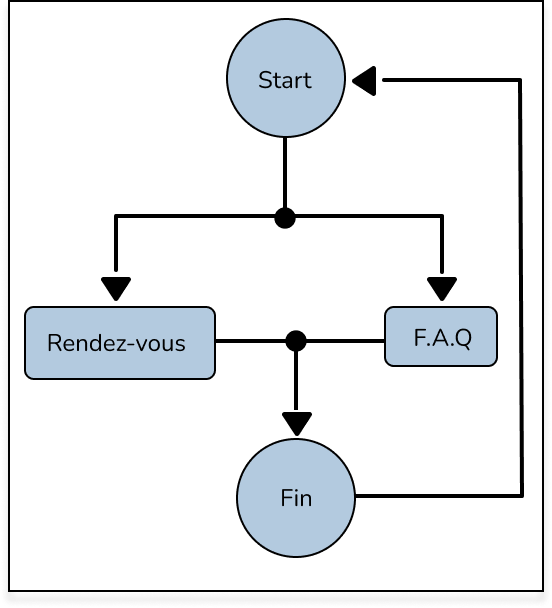
\includegraphics[scale=0.8]{Figures/cbf_overall.png}
    \caption{Flux général du Chatbot}
\end{figure}

% [width=8cm]
\subsection{FAQ}

\hspace{16pt}Le chatbot propose à l'utilisateur des sujets prédéfinis sur lesquels il pourrait vouloir en savoir plus, et lors de la sélection d'un, le chatbot répond avec une réponse prédéfinie.

\begin{figure}[H] 
    \centering
    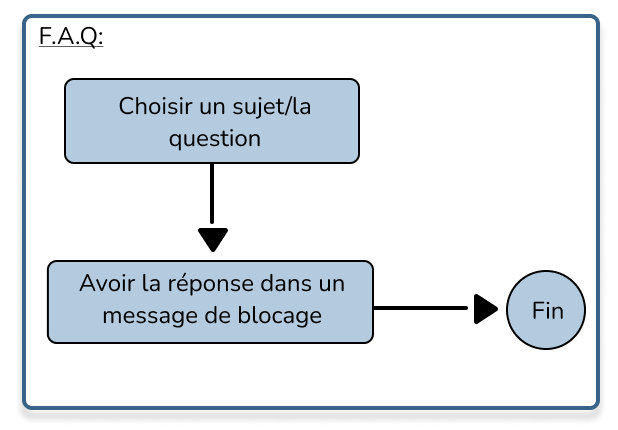
\includegraphics[scale=0.8]{Figures/cbf_faq.png}
    \caption{Flux du processus: F.A.Q}
\end{figure}

\subsection{Prise de rendez-vous}

\hspace{16pt}Le chatbot guide l'utilisateur avec un flux prédéfini dans ce cas, depuis la demande d'informations de base sur l'utilisateur jusqu'aux opérations facultatives telles que répondre à des questions spécialisées ou joindre des documents, avec une validation intégrée pour chaque petite information que nous lui demandons de fournir (si la validation est possible dans le premier lieu).


\begin{figure}[H] 
    \centering
    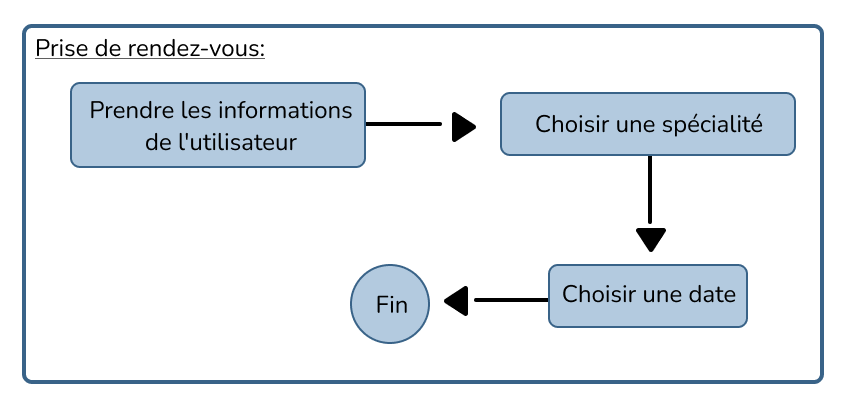
\includegraphics[scale=0.8]{Figures/cbf_rdv.png}
    \caption{Flux du processus: Prise de rendez-vous}
\end{figure}


\begin{figure}[H] 
    \centering
    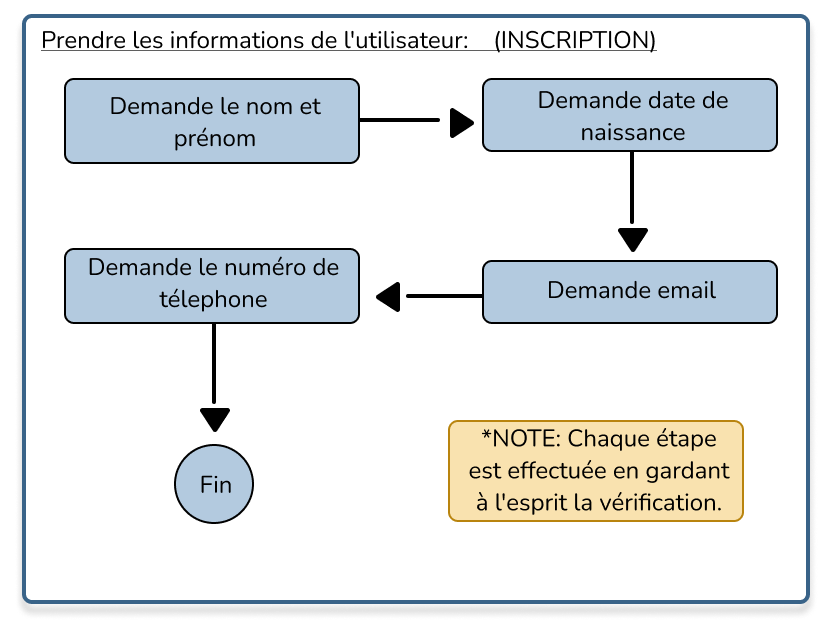
\includegraphics[scale=0.8]{Figures/cbf_user.png}
    \caption{Flux du processus: Prise de rendez-vous (Prendre les informations de l'utilisateur)}
\end{figure}


\begin{figure}[H] 
    \centering
    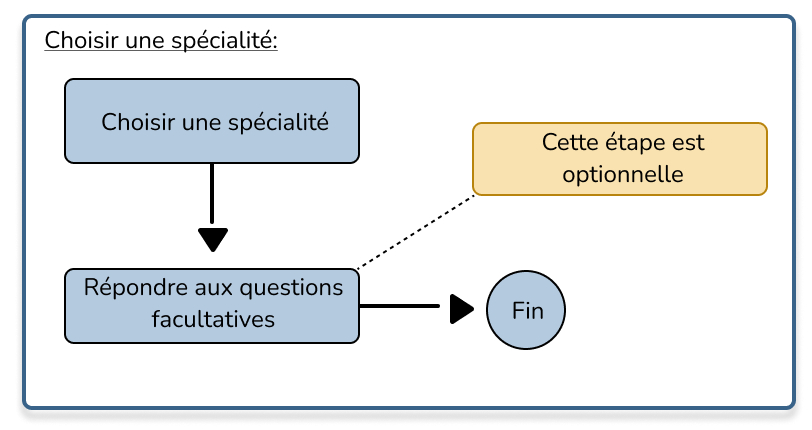
\includegraphics[scale=0.9]{Figures/cbf_specialite.png}
    \caption{Flux du processus: Prise de rendez-vous (Choisir une spécialité)}
\end{figure}


\section{Explication des choix technologiques}

\hspace{16pt}Pour les technologies, nous n'avions pas beaucoup de choix, on nous proposait de travailler soit avec Django de Python, soit avec React (Front-end) et Symfony* (Back-end).

\subsection{React}


\subsubsection{Interface Utilisateur Réactive et Performante}

\begin{itemize}
  \item \textbf{DOM Virtuel: }React utilise un DOM virtuel pour des mises à jour rapides et efficaces de l'interface utilisateur, garantissant une expérience utilisateur fluide et sans latence.
  \item \textbf{Rendu Dynamique: }Les capacités de rendu dynamique de React permettent de gérer efficacement les interactions en temps réel, cruciales pour un chatbot.
\end{itemize}

\subsubsection{Composants Réutilisables et Modulaire}
 
\begin{itemize}
  \item \textbf{Composants: }La structure basée sur les composants de React facilite la création de widgets et de modules réutilisables pour différentes parties du chatbot, comme les fenêtres de conversation, les formulaires de saisie, et les notifications.
  \item \textbf{Modularité: }Permet de construire l'application de manière modulaire, rendant le code plus maintenable et évolutif.
\end{itemize}

\subsubsection{Intégration Facile avec les APIs}

\begin{itemize}
  \item \textbf{Hooks: }Les hooks de React, comme useEffect et useState, simplifient les appels API et la gestion des états, permettant une intégration fluide avec les services backend du chatbot.
  \item \textbf{Interopérabilité: }React facilite l'intégration avec des APIs RESTful ou GraphQL, nécessaires pour les fonctionnalités de traitement du langage naturel (NLP) et la gestion des dialogues.
\end{itemize}

\subsubsection{Écosystème et Communauté}

\begin{itemize}
  \item \textbf{Support et Documentation: }La vaste communauté de React et sa documentation exhaustive offrent un soutien continu et des ressources abondantes pour résoudre les problèmes et optimiser le développement.
  \item \textbf{Outils et Bibliothèques: }Un large éventail de bibliothèques et d'outils complémentaires, tels que les bibliothèques de calendriers et même la bibliothèque de chatbots avec laquelle nous avons travaillé.
\end{itemize}


\subsection{Symfony}


\subsubsection{Framework PHP Puissant}

\begin{itemize}
  \item Symfony est un framework PHP mature et puissant, offrant une structure solide et bien organisée pour le développement d'applications web complexes telles que le chatbot médical. Sa stabilité et sa maturité en font un choix fiable pour la création d'un back-end robuste.
\end{itemize}

\subsubsection{Gestion de l'API avec API Platform}

\begin{itemize}
  \item Symfony offre une intégration transparente avec API Platform, une solution robuste pour la création et la gestion d'API RESTful. En configurant l'API avec Symfony et API Platform, nous bénéficions d'une documentation automatique, d'une gestion avancée des opérations CRUD, et d'une sérialisation/désérialisation automatique des données.
\end{itemize}

\subsubsection{Sécurité Renforcée}

\begin{itemize}
  \item Symfony intègre des fonctionnalités avancées de sécurité, telles que la protection contre les attaques CSRF, XSS et SQL injection. Cela garantit un niveau élevé de sécurité pour les données sensibles des utilisateurs du chatbot médical, ce qui est essentiel dans le domaine médical.
\end{itemize}


\section{Diagrammes de conception utilisés}

\hspace{16pt}Dans le cadre du développement du chatbot pour la maison médicale, nous avons créé un Modèle Conceptuel de Données (MCD) pour concevoir la structure de la base de données. Le MCD ci-dessous illustre les principales entités et leurs relations dans notre système.\\


\begin{figure}[H] 
    \centering
    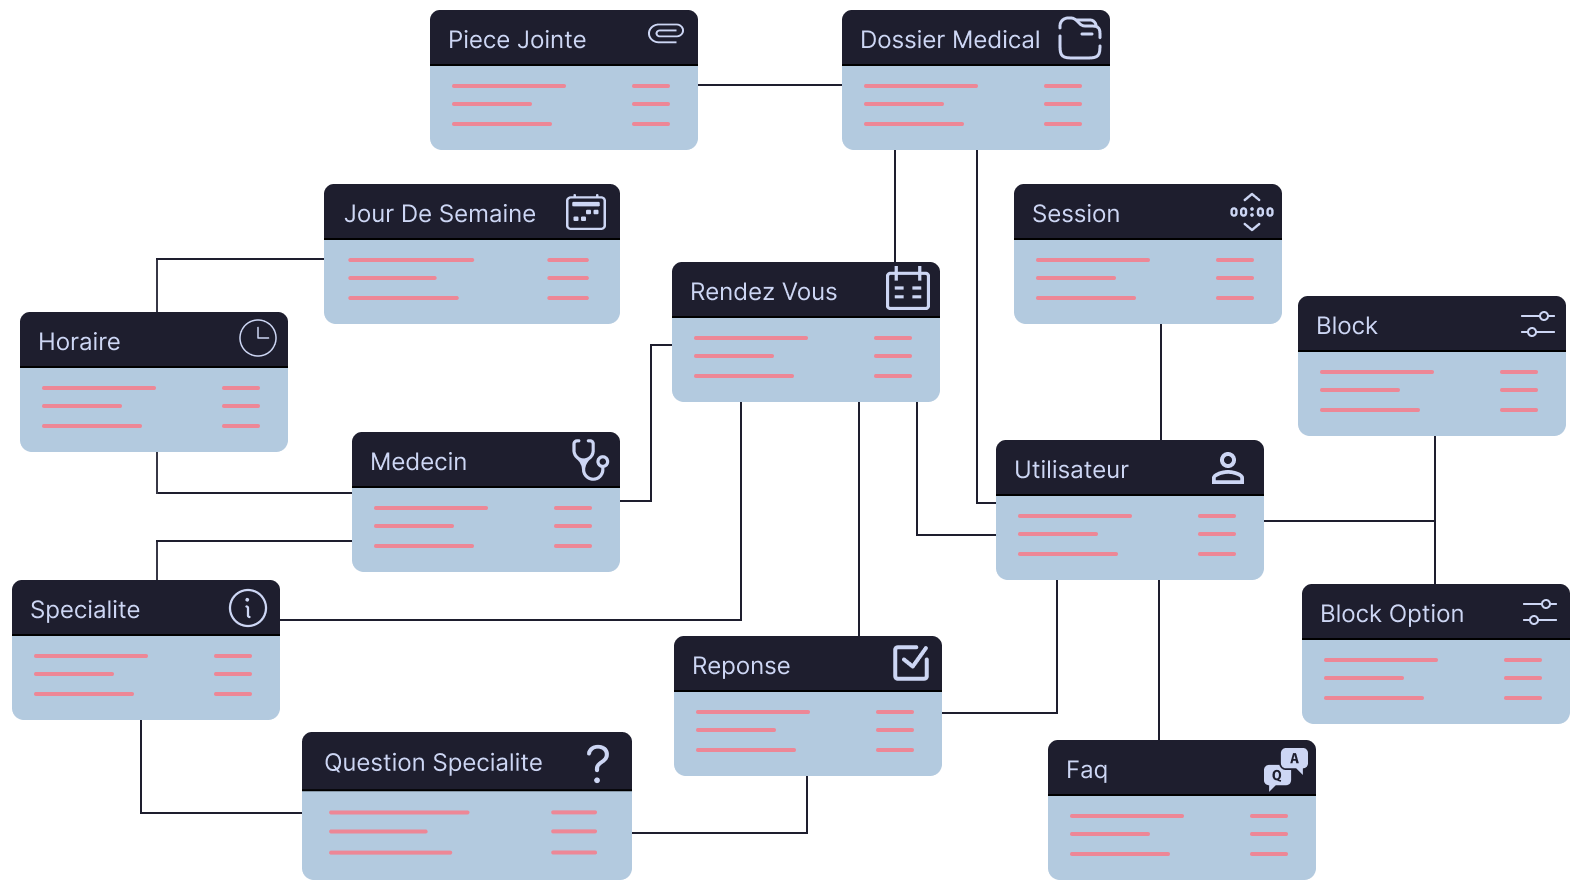
\includegraphics[scale=0.67]{Figures/MCD.png}
    \caption{Diagramme de conception}
    \label{entite} %Optional (If you want to reference the figure in later chapters)
\end{figure}

Ce MCD représente les principales entités de notre base de données pour le chatbot médical. Voici une brève explication de chaque entité :


\begin{itemize}
  \item \textbf{Utilisateur: }Stocke les informations sur les utilisateurs du chatbot, telles que leur identifiant, leur nom et leurs informations de contact. Les utilisateurs peuvent avoir des rôles spécifiques, comme patient ou admin.
  \item \textbf{Medecin: }Stocke les informations sur les médecins, telles que leur identifiant, leur nom et leurs informations de contact.
  \item \textbf{Specialite: }Décrit les différentes spécialités médicales disponibles, telles que la cardiologie, la dermatologie, etc.
  \item \textbf{Question Specialite: }Contient des questions uniques pour chaque spécialité.
  \item \textbf{Reponse: }Enregistre les réponses fournies par les patients aux questions relatives à une spécialité médicale. Inclut des références à l'utilisateur, à la question de spécialité et à la réponse fournie.
  \item \textbf{Jour De Semaine: }Stocke les jours de la semaine pour aider à gérer les horaires et les disponibilités des médecins et des rendez-vous.
  \item \textbf{Horaire: }Définit les plages horaires disponibles pour les rendez-vous et les sessions avec les médecins.
  \item \textbf{Session: }Contient la séance de travail pour le centre médical.
  \item \textbf{Rendez Vous: }Enregistre les rendez-vous programmés, y compris la date, l'heure, le patient et le médecin assigné.
  \item \textbf{Faq: }Stocke les questions fréquentes et leurs réponses associées, utilisées par le chatbot pour fournir des informations instantanées.
  \item \textbf{Block: }Décrit les blocs de contenu ou de dialogue utilisés dans le chatbot pour structurer les conversations.
  \item \textbf{Block Option: }Contient les options disponibles pour chaque bloc de contenu, permettant au chatbot de guider les utilisateurs à travers différentes branches de la conversation.
  \item \textbf{Piece jointe: }Gère le téléchargement de fichiers. Cette entité stocke les informations sur les fichiers joints aux conversations.
  \item \textbf{Dossier Medical: }Gère les dossiers médicaux des utilisateurs. Cette entité permet le téléchar-gement de plusieurs fichiers pour chaque utilisateur.
\end{itemize}



\newpage

\section*{Conclusion}

\hspace{16pt}La conception et le développement de l'application décrits dans ce chapitre montrent comment les choix technologiques et les approches méthodologiques ont permis de créer une solution efficace et robuste. En utilisant des frameworks modernes et des pratiques de conception bien établies, nous avons pu développer une application qui répond aux besoins des utilisateurs de manière optimale.

\pagebreak
